\begin{document}

\ThesisStart{male}
%\ThesisStart{zadani-a-prohlaseni.pdf}

\begin{abstractCZ}
Český abstrakt
\end{abstractCZ}

\begin{keywordsCZ}
Klíčová slova česky
\end{keywordsCZ}

\vspace{2cm}

\begin{abstractEN}
English abstract
\end{abstractEN}

\begin{keywordsEN}
keywords in English
\end{keywordsEN}

\begin{acknowledgement}
\end{acknowledgement}

\tableofcontents

\clearpage

\begin{acronym}[MPSoC] % To v závorce určuje odsazení (dej sem nejdelší zkratku)
    \acro{APU}{Application Processing Unit}
    \acro{AXI}{Advanced eXtensible Interface}
    \acro{BRAM}{Block Random Access Memory}
    \acro{DMA}{Direct Memory Access}
    \acro{DSP}{Digital Signal Processing}
    \acro{FPGA}{Field Programmable Gate Array}
    \acro{HLS}{High-Level Synthesis}
    \acro{IP}{Intellectual Property}
    \acro{LUT}{Look-Up Table}
    \acro{MIPI}{Mobile Industry Processor Interface}
    \acro{MPSoC}{Multiprocessor System on Chip}
    \acro{PL}{Programmable Logic}
    \acro{PS}{Processing System}
    \acro{RTL}{Register Transfer Level}
    \acro{SoC}{System on Chip}
    \acro{SOM}{System-on-Module}
    \acro{VHDL}{VHSIC Hardware Description Language}
    \acro{VHSIC}{Very High Speed Integrated Circuit}
\end{acronym}


\begin{abbrList}
\textbf{APU} & Application Processing Unit \\
\textbf{AXI} & Advanced eXtensible Interface \\
\textbf{BRAM} & Block Random Access Memory \\
\textbf{DMA} & Direct Memory Access \\
\textbf{DSP} & Digital Signal Processing \\
\textbf{FPGA} & Field Programable Gate Array \\
\textbf{HLS} & High Level Synthesis \\
\textbf{IP} & Intellectual Property \\
\textbf{LUT} & Look-Up Table \\
\textbf{MIPI} & Mobile Industry Processor Interface \\
\textbf{MPSoC} & Multiprocessor System on Chip \\
\textbf{PL} & Programmable Logic \\
\textbf{PS} & Processing System \\
\textbf{RTL} & Register Transfer Level \\
\textbf{SoC} & System on Chip \\
\textbf{SOM} & System-on-Module \\
\textbf{VHDL} & VHSIC Hardware Description Language \\
\textbf{VHSIC} & Very High Speed Integrated Circuit \\
\end{abbrList}


\chapter{Úvod}


\chapter{Nástroje}

\section{AMD Vitis™ HLS for Intuitive Design and Productivity}

\textbf{AMD Vitis™ HLS} je pokročilý vývojový nástroj určený pro automatizovanou syntézu digitálního hardwaru z vysokoúrovňových programovacích jazyků.\\Tento nástroj umožňuje transformaci algoritmického popisu v jazycích C/C++ do nízkoúrovňového RTL popisu, typicky ve VHDL nebo Verilogu, optimalizovaného pro FPGA a adaptivní SoC platformy společnosti AMD.
\\
\\
V kontextu návrhu systémů pro zpracování obrazu představuje Vitis HLS klíčový prvek, který abstrahuje komplexitu hardwarového návrhu a umožňuje soustředit se na funkční stránku algoritmů. Nástroj provádí automatickou analýzu kódu, plánování (scheduling) a mapování operací na dostupné hardwarové zdroje (DSP bloky, paměťové bloky).

Mezi klíčové vlastnosti, využívané v této práci, patří:

\begin{itemize}
    \item \textbf{Hardwarová akcelerace:} Generování vysoce optimalizovaných IP jader (Intellectual Property cores) s možností definovat výkonnostní parametry, jako je propustnost a latence.
    
    \item \textbf{Optimalizační direktivy:} Využití tzv. pragmas pro řízení architektury výsledného hardwaru, včetně paralelizace smyček (loop unrolling), pipeliningu instrukcí a správy paměťových rozhraní.
    
    \item \textbf{Verifikace:} Integrované prostředí pro C-simulaci (ověření funkčnosti algoritmu) a C/RTL ko-simulaci (ověření bitové shody vygenerovaného RTL s původním C++ modelem).

    \item \textbf{Integrace:} Přímá návaznost na sadu AMD Vivado™ Design Suite pro finální implementaci, syntézu a nahrání bitstreamu do cílového zařízení, např. kitu Kria KV260. a  \cite{amd_vitis}
\end{itemize}

\newpage

\section{AMD Vivado™ Design Suite}
\textbf{AMD Vivado™} je komplexní integrované vývojové prostředí pro SOC a FPGA. Které obsahuje: návrh, syntézu, plánování a mapování, verifikační a simulační nástroje. 

Pro účely této práce slouží Vivado jako centrální integrační platforma, která propojuje hardwarové akcelerátory vyvinuté v nástroji Vitis HLS s procesorovým subsystémem (PS) platformy Kria KV260. Klíčovou komponentou prostředí je nástroj IP Integrator, který umožňuje grafický návrh systému na úrovni bloků (Block Design). Zde jsou jednotlivá IP jádra (Intellectual Property cores) propojena pomocí standardizované sběrnice AMBA® AXI, což zajišťuje efektivní komunikaci mezi programovatelnou logikou a řídicím procesorem ARM.

Proces návrhu ve Vivado Design Suite zahrnuje následující klíčové fáze:

\begin{itemize}
    \item \textbf{RTL Syntéza:} Převod zdrojových kódů (VHDL, Verilog) a blokových schémat do seznamu spojů (netlist).
    
    \item \textbf{Implementace:} Fyzický návrh čipu zahrnující rozmístění (Placement) logických elementů a propojení (Routing) signálových tras. Moderní verze Vivado ML (Machine Learning) využívají v této fázi algoritmy strojového učení pro optimalizaci časování a minimalizaci spotřeby.
    
    \item \textbf{Verifikace:} Ověření funkčnosti návrhu pomocí behaviorální a post-implementační simulace.
    
    \item \textbf{Generování bitstreamu:} Vytvoření konfiguračního souboru pro FPGA část a export hardwarové definice (XSA soubor) pro následný vývoj softwaru.
\end{itemize}

Součástí prostředí je také Vivado Hardware Manager, který umožňuje programování cílového zařízení přes rozhraní JTAG a ladění běžícího hardwaru v reálném čase pomocí integrovaných logických analyzátorů (ILA - Integrated Logic Analyzer).

\section{Vývojová deska kria KV260 Vision AI Starter Kit}

\textbf{xck26-sfvc784-2lv-c
}
AMD Kria™ KV260 Vision AI Starter Kit je navržená jako výuková platforma pro návrh a vývoj pokročilých aplikací počítačového vidění se zaměřením na akceleraci vizuálních algoritmů a strojového učení. Tento kit je založen na architektuře \textbf{Zynq® UltraScale+™ MPSoC} a skládá se z v neprodukčního modulu Kria K26 SOM (System-on-Module) osazeného na nosné desce (carrier card) s bohatou sadou rozhraní pro připojení více kamer a zobrazovacích zařízení pomocí konektoru ON Semiconductor Imager Access System (IAS).
Platforma je určena primárně pro vývoj řešení v oblastech, jako jsou chytrá města, průmyslové vidění (machine vision) a bezpečnostní kamery. Díky integrovanému video kodeku (VCU) a programovatelné logice na FPGA umožňuje hardwarovou akceleraci celého aplikačního řetězce – od snímání obrazu přes jeho zpracování až po inferenci neuronových sítí, a to při zachování nízké spotřeby energie a latence. \cite{amd_kv260}

\begin{table}[htbp]
    \centering
    \caption{Technická specifikace vývojové desky AMD Kria KV260 Vision AI Starter Kit \cite{amd_kv260}}
    \label{tab:kv260-specs}
    \begin{tabular}{@{}ll@{}}
        \toprule
        \textbf{Komponenta / Rozhraní} & \textbf{Specifikace} \\ \midrule
        SoC (Čip) & Zynq™ UltraScale+™ MPSoC (modul K26 SOM) \\
        Obrazový procesor & OnSemi AP1302 13MP ISP\\
        Programovatelná logika & 256 tisíc logických buněk,
144 bloků RAM
64 bloků UltraRAM
1 176 DSP slices\\
        Paměť DRR& 4 GB (4 x 512 Mb x 16 bit)\\
        Kamerová rozhraní & 3$\times$ MIPI CSI-2 (2$\times$ IAS, 1$\times$ RPi) \\
        Video výstupy & 1$\times$ HDMI 1.4, 1$\times$ DisplayPort 1.2a\\
        Síťové rozhraní & 1$\times$ 1Gb Ethernet \\
        Rozšiřující rozhraní & 1$\times$ PMOD (12-pin) \\
        USB & 4$\times$ USB 3.0/2.0 \\
        Úložiště dat & Primární  - 512 Mb QSPI (Queued SPI)
Sekundární - slot pro SDHC kartu\\
    \end{tabular}
\end{table}

\chapter{Zpracování obrazových dat}
\section{Převody barevných prostorů}

\subsection{RGB a sRGB}

\subsection{RGB na HSV}

\[
\begin{aligned}
R' &= \frac{R}{255}, \quad G' = \frac{G}{255}, \quad B' = \frac{B}{255} \\
C_{max} &= \max(R', G', B') \\
C_{min} &= \min(R', G', B') \\
\Delta &= C_{max} - C_{min} \\
\\
H &= \begin{cases} 
0^\circ & \Delta = 0 \\
60^\circ \times \left(\frac{G' - B'}{\Delta} \pmod 6\right) & C_{max} = R' \\
60^\circ \times \left(\frac{B' - R'}{\Delta} + 2\right) & C_{max} = G' \\
60^\circ \times \left(\frac{R' - G'}{\Delta} + 4\right) & C_{max} = B'
\end{cases} \\
\\
S &= \begin{cases} 
0 & C_{max} = 0 \\
\frac{\Delta}{C_{max}} & C_{max} \neq 0 
\end{cases} \\
\\
V &= C_{max}
\end{aligned}
\]



a zpětná transformace 

\[\begin{aligned}
C &= V \times S \\
X &= C \times (1 - |(H / 60^\circ) \pmod 2 - 1|) \\
m &= V - C \\
\\
(R', G', B') &= \begin{cases} 
(C, X, 0) & 0^\circ \le H < 60^\circ \\
(X, C, 0) & 60^\circ \le H < 120^\circ \\
(0, C, X) & 120^\circ \le H < 180^\circ \\
(0, X, C) & 180^\circ \le H < 240^\circ \\
(X, 0, C) & 240^\circ \le H < 300^\circ \\
(C, 0, X) & 300^\circ \le H < 360^\circ
\end{cases} \\
\\
R &= (R' + m) \times 255 \\
G &= (G' + m) \times 255 \\
B &= (B' + m) \times 255 
\end{aligned}\]

\section{Barevný prostor YUV a jeho využití}

Lidský zrakový systém (HVS -- \textit{Human Visual System}) je evolučně uzpůsoben tak, že vykazuje podstatně vyšší citlivost na změny jasu (luminance) než na změny barvy (chrominance). Zatímco barevný prostor RGB je ideální pro zobrazení na koncových zařízeních (monitory, displeje), pro účely zpracování, přenosu a komprese obrazu je krajně neefektivní kvůli vysoké korelaci mezi jednotlivými barevnými kanály. Z tohoto důvodu byl definován barevný prostor YUV, který jasovou a barevnou informaci odděluje.

Obecný výpočetní vzorec:
\begin{equation}
\begin{aligned}
    Y = Y_R \cdot R + Y_G \cdot G + Y_B \cdot B \\
    \text{přičemž platí:} \quad Y_R + Y_G + Y_B &= 1 \\[10pt]
    \text{Odvození } P_B \text{ a } P_R \text{:} \qquad P_B &= 1 - Y_B \\
    P_R &= 1 - Y_R \\[10pt]
    C_B &= \frac{B - Y}{2P_B} \\
    C_R &= \frac{R - Y}{2P_R}
\end{aligned}
\end{equation}

\subsection{Definice složek Y, U a V}

Prostor YUV transformuje obraz do jedné jasové a dvou barvonosných (rozdílových) složek. Toto rozdělení vychází z historických potřeb zpětné kompatibility barevného televizního vysílání s černobílými přijímači a je zakotveno ve standardech Mezinárodní telekomunikační unie (ITU).

\begin{itemize}
    \item \textbf{Y (Jasová složka / Luma):} Reprezentuje monochromatickou (černobílou) verzi obrazu. Udává úroveň jasu každého pixelu nezávisle na jeho barvě.
    \item \textbf{U (Chrominance B-Y):} Barevná rozdílová složka reprezentující odchylku modré barvy od celkového jasu.
    \item \textbf{V (Chrominance R-Y):} Barevná rozdílová složka reprezentující odchylku červené barvy od celkového jasu.
\end{itemize}

Rozdílová složka zelené barvy (G-Y) se nepřenáší, jelikož ji lze matematicky odvodit ze složek Y, U a V, čímž se šetří datový tok.

\subsection{Matematické matice převodu z RGB}

Převod mezi prostory RGB a YUV není fixní, nýbrž závisí na váhových koeficientech definujících příspěvek jednotlivých základních barev do celkového jasu. Tyto koeficienty se vyvíjely v závislosti na použitých luminoforech a moderních zobrazovacích technologiích. Ve všech případech se však vychází z normovaných hodnot $R, G, B \in [0, 1]$.

\subsubsection{Standard ITU-R BT.601 (SDTV)}
Tento standard byl primárně definován pro televizi se standardním rozlišením (SDTV). Matice pro dopřednou transformaci z RGB do YUV je definována následovně:

\begin{equation}
\begin{pmatrix}
Y \\
U \\
V
\end{pmatrix}
=
\begin{pmatrix}
0.299 & 0.587 & 0.114 \\
-0.14713 & -0.28886 & 0.436 \\
0.615 & -0.51499 & -0.10001
\end{pmatrix}
\begin{pmatrix}
R \\
G \\
B
\end{pmatrix}
\label{eq:bt601}
\end{equation}

\subsubsection{Standard ITU-R BT.709 (HDTV)}
S nástupem televize s vysokým rozlišením (HDTV) byly koeficienty upraveny tak, aby lépe odpovídaly moderním displejům. Zejména se snížil váhový příspěvek červené a modré složky ve prospěch zelené:

\begin{equation}
\begin{pmatrix}
Y \\
U \\
V
\end{pmatrix}
=
\begin{pmatrix}
0.2126 & 0.7152 & 0.0722 \\
-0.09991 & -0.33609 & 0.436 \\
0.615 & -0.55861 & -0.05639
\end{pmatrix}
\begin{pmatrix}
R \\
G \\
B
\end{pmatrix}
\label{eq:bt709}
\end{equation}

\subsection{Standard ITU-R BT.2020 (UHDTV)}

\begin{equation}
\begin{pmatrix}
Y \\
U \\
V
\end{pmatrix}
=
\begin{pmatrix}
 0.2627 &  0.6780 &  0.0593 \\
-0.1396 & -0.3604 &  0.5000 \\
 0.5000 & -0.4598 & -0.0402
\end{pmatrix}
\begin{pmatrix}
R \\
G \\
B
\end{pmatrix}
\label{eq:bt2020}
\end{equation}

\begin{table}[htbp]
\centering
\caption{Porovnání primárních převodových koeficientů jasové složky pro standardy ITU-R.}
\begin{tabular}{lccc}
\toprule
\textbf{Standard} & $\mathbf{W_R}$ (Váha červené) & $\mathbf{W_G}$ (Váha zelené) & $\mathbf{W_B}$ (Váha modré) \\
\midrule
ITU-R BT.601 (SD)  & 0.2990  & 0.5870  & 0.1140 \\
ITU-R BT.709 (HD)  & 0.2126  & 0.7152  & 0.0722 \\
ITU-R BT.2020 (4K) & 0.2627  & 0.6780  & 0.0593 \\
\bottomrule
\end{tabular}
\label{tab:yuv_coeffs}
\end{table}

\subsection{Diagram U-V barevné roviny}

Vztah mezi jasem a barvou lze vizualizovat v tzv. U-V rovině (při konstantním jasu Y). Na obrázku \ref{fig:uv_plane} je zobrazen vektorový prostor chrominančních složek s vyznačením polohy primárních (RGB) a sekundárních (CMY) barev dle standardu BT.601.

\begin{figure}[htbp]
\centering
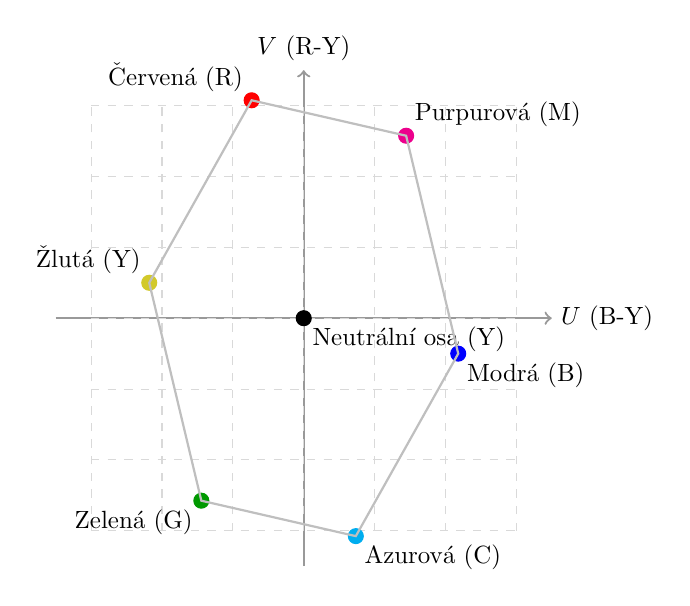
\begin{tikzpicture}[scale=4.5, every node/.style={scale=0.9}]
    % Osy
    \draw[->, thick, gray!80] (-0.7, 0) -- (0.7, 0) node[right, text=black] {$U$ (B-Y)};
    \draw[->, thick, gray!80] (0, -0.7) -- (0, 0.7) node[above, text=black] {$V$ (R-Y)};
    
    % Mrizka
    \draw[dashed, gray!30, step=0.2] (-0.6,-0.6) grid (0.6,0.6);
    
    % Body barev BT.601 (Y,U,V)
    % Red: U=-0.147, V=0.615
    \filldraw[red] (-0.147, 0.615) circle (0.6pt) node[above left, text=black] {Červená (R)};
    % Green: U=-0.289, V=-0.515
    \filldraw[green!60!black] (-0.289, -0.515) circle (0.6pt) node[below left, text=black] {Zelená (G)};
    % Blue: U=0.436, V=-0.100
    \filldraw[blue] (0.436, -0.100) circle (0.6pt) node[below right, text=black] {Modrá (B)};
    
    % Cyan: U=0.147, V=-0.615
    \filldraw[cyan] (0.147, -0.615) circle (0.6pt) node[below right, text=black] {Azurová (C)};
    % Magenta: U=0.289, V=0.515
    \filldraw[magenta] (0.289, 0.515) circle (0.6pt) node[above right, text=black] {Purpurová (M)};
    % Yellow: U=-0.436, V=0.100
    \filldraw[yellow!80!black] (-0.436, 0.100) circle (0.6pt) node[above left, text=black] {Žlutá (Y)};
    
    % Pocatek (šedá/bílá/černá - žádná barevná informace)
    \filldraw[black] (0, 0) circle (0.6pt) node[below right] {Neutrální osa (Y)};
    
    % Polygon hranice
    \draw[thick, gray!50] (-0.147, 0.615) -- (0.289, 0.515) -- (0.436, -0.100) -- (0.147, -0.615) -- (-0.289, -0.515) -- (-0.436, 0.100) -- cycle;

\end{tikzpicture}
\caption{Projekce barevného prostoru do 2D chrominanční roviny U-V (tzv. YUV gamut). Neutrální barvy (odstíny šedi) leží v počátku souřadnic (U=0, V=0).}
\label{fig:uv_plane}
\end{figure}

\subsection{Chrominanční podvzorkování (Chroma Subsampling)}

Jedním z nejzásadnějších důvodů pro přechod z RGB do YUV v oblasti zpracování obrazu je možnost provedení tzv. \textit{chrominančního podvzorkování} (chroma subsampling). Vzhledem ke zmíněné nižší citlivosti lidského oka na barvu lze prostorové rozlišení složek U a V redukovat, aniž by pozorovatel zaznamenal zjevnou degradaci obrazové kvality.

Systém zápisu podvzorkování se nejčastěji vyjadřuje poměrem $J:a:b$, kde $J$ je šířka referenčního bloku (obvykle 4 pixely), $a$ je počet vzorků chrominance v prvním řádku a $b$ počet vzorků chrominance ve druhém řádku.

\begin{figure}[htbp]
\centering
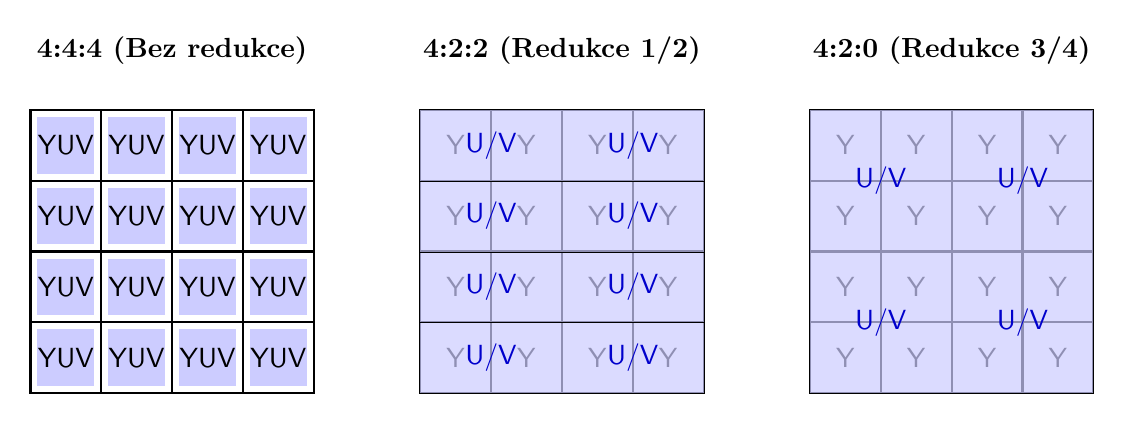
\begin{tikzpicture}[scale=0.9, font=\sffamily]

    % Format 4:4:4
    \begin{scope}[xshift=0cm]
        \node[above, font=\bfseries] at (2, 4.5) {4:4:4 (Bez redukce)};
        \foreach \y in {0,1,2,3} {
            \foreach \x in {0,1,2,3} {
                % Y sample
                \draw[thick] (\x, \y) rectangle ++(1,1);
                % U/V sample matches Y
                \fill[blue!20] (\x+0.1, \y+0.1) rectangle ++(0.8,0.8);
                \node at (\x+0.5, \y+0.5) {YUV};
            }
        }
    \end{scope}

    % Format 4:2:2
    \begin{scope}[xshift=5.5cm]
        \node[above, font=\bfseries] at (2, 4.5) {4:2:2 (Redukce 1/2)};
        \foreach \y in {0,1,2,3} {
            \foreach \x in {0,1,2,3} {
                \draw[thick] (\x, \y) rectangle ++(1,1);
                \node at (\x+0.5, \y+0.5) {Y};
            }
            \foreach \x in {0,2} {
                \fill[blue!20, opacity=0.7] (\x, \y) rectangle ++(2,1);
                \node[blue!80!black] at (\x+1, \y+0.5) {U/V};
            }
        }
    \end{scope}

    % Format 4:2:0
    \begin{scope}[xshift=11cm]
        \node[above, font=\bfseries] at (2, 4.5) {4:2:0 (Redukce 3/4)};
        \foreach \y in {0,1,2,3} {
            \foreach \x in {0,1,2,3} {
                \draw[thick] (\x, \y) rectangle ++(1,1);
                \node at (\x+0.5, \y+0.5) {Y};
            }
        }
        \foreach \y in {0,2} {
            \foreach \x in {0,2} {
                \fill[blue!20, opacity=0.7] (\x, \y) rectangle ++(2,2);
                \node[blue!80!black] at (\x+1, \y+1) {U/V};
            }
        }
    \end{scope}

\end{tikzpicture}
\caption{Vizualizace principu chrominančního podvzorkování. Každý čtverec v mřížce představuje jeden pixel. Jasová složka (Y) je zachována vždy v plném rozlišení, zatímco barevná informace (U/V) je sdílena pro více sousedících pixelů.}
\label{fig:subsampling}
\end{figure}

\subsection{Výhody pro kompresi a zpracování obrazu}

Transformace do prostoru YUV poskytuje pro moderní systémy počítačového vidění a kompresní algoritmy (např. JPEG, H.264/AVC, HEVC) následující klíčové benefity:

\begin{enumerate}
    \item \textbf{Datová úspora bez vizuální ztráty:} Aplikací podvzorkování 4:2:0 dochází k redukci celkového objemu dat nekomprimovaného obrazu na polovinu oproti původnímu RGB formátu, a to ještě před aplikací samotných kompresních algoritmů (např. diskrétní kosinové transformace DCT).
    \item \textbf{Energetická efektivita algoritmů:} Mnoho algoritmů zpracování obrazu (detekce hran, sledování pohybu, extrakce příznaků) nevyžaduje barevnou informaci. Namísto konverze celého RGB obrazu na černobílý stačí v systému YUV pouze vyextrahovat existující kanál Y a provést výpočty nad ním.
    \item \textbf{Optimalizace kvantizace:} Během kompresního procesu (např. v normě JPEG) jsou používány rozdílné kvantizační matice pro jas a pro barvu. Matice aplikované na chrominanční kanály odstraňují podstatně více vysokofrekvenčních detailů (agresivnější ztrátová komprese) než u kanálu jasového.
\end{enumerate}


dle standardu \textbf{SDTV ITU-R BT.601}
dle standardu \textbf{SDTV ITU-R BT.709} FULL HP
dle standardu \textbf{SDTV ITU-R BT.2020} 4K (možná až 8?)

\[\begin{aligned}
Y &= 0.299R + 0.587G + 0.114B \\
U &= -0.14713R - 0.28886G + 0.436B \\
V &= 0.615R - 0.51499G - 0.10001B
\end{aligned}\]

zpětný převod dostaneme inverzní maticí

\[\begin{aligned}
R &= Y + 1.13983V \\
G &= Y - 0.39465U - 0.58060V \\
B &= Y + 2.03211U
\end{aligned}\]

\subsection{RGB na YUV}
\subsection{}

\section{Histogram}

\href{https://docs.opencv.org/3.4/d4/d1b/tutorial_histogram_equalization.html}{Histogram opencv}
\section{Filtrace}

https://opencv.org/image-filtering-using-convolution-in-opencv/

% Requires: \usepackage{amsmath}
\begin{equation}
    (f * g)(x, y) = \sum_{m=-\infty}^{\infty} \sum_{n=-\infty}^{\infty} f(m, n)\, g(x - m, y - n)
    \label{eq:placeholder_label}
\end{equation}

Ztráta okrajů a zpoždění (Flushing): Pokud chceme režim SAME (výstupní obraz je stejně velký jako vstupní), okno začne generovat platný středový pixel až ve chvíli, kdy do něj nateče celá polovina jádra. Abychom na konci obrazu ze systému "vytlačili" i ty úplně poslední pixely, musí pipelina běžet o něco déle, než je počet pixelů v obraze. Tomuto se říká Flushing.

Identita
\begin{equation}
    \begin{bmatrix}
        0 & 0 & 0 \\
        0 & 1 & 0 \\
        0 & 0 & 0
    \end{bmatrix}
\end{equation}

\subsection{Průměrovací filtr}
Průměrovací filtr
\begin{equation}
    \frac{1}{9} \cdot 
    \begin{bmatrix}
        1 & 1 & 1 \\
        1 & 1 & 1 \\
        1 & 1 & 1
    \end{bmatrix}
\end{equation}

Zostřovací filtr
\begin{equation}
    \begin{bmatrix}
        0 & -1 & 0 \\
        -1 & 5 & -1 \\
        0 & -1 & 0
    \end{bmatrix}
\end{equation}

\subsection{Hranové filtry}

Prewitt horizontální
\begin{equation}
    \begin{bmatrix}
        -1 & 0 & 1 \\
        -1 & 0 & 1 \\
        -1 & 0 & 1
    \end{bmatrix}
\end{equation}

Prewitt vertikální
\begin{equation}
    \begin{bmatrix}
        -1 & -1 & -1 \\
        0 & 0 & 0 \\
        1 & 1 & 1
    \end{bmatrix}
\end{equation}

Sobel horizontální
\begin{equation}
    \begin{bmatrix}
        -1 & 0 & 1 \\
        -2 & 0 & 2 \\
        -1 & 0 & 1
    \end{bmatrix}
\end{equation}

Sobel vertikální
\begin{equation}
    \begin{bmatrix}
        -1 & -2 & -1 \\
        0 & 0 & 0 \\
        1 & 2 & 1
    \end{bmatrix}
\end{equation}

\subsection{Morfologické operace}

V morfologii se tyto matice označují jako strukturní prvky ($S$).

Čtvercový element ($3 \times 3$)
\begin{equation}
    S_{square} = \begin{bmatrix}
        1 & 1 & 1 \\
        1 & 1 & 1 \\
        1 & 1 & 1
    \end{bmatrix}
\end{equation}

Křížový element ($3 \times 3$)
\begin{equation}
    S_{cross} = \begin{bmatrix}
        0 & 1 & 0 \\
        1 & 1 & 1 \\
        0 & 1 & 0
    \end{bmatrix}
\end{equation}

Aproximace disku ($5 \times 5$)
\begin{equation}
    S_{disk} = \begin{bmatrix}
        0 & 0 & 1 & 0 & 0 \\
        0 & 1 & 1 & 1 & 0 \\
        1 & 1 & 1 & 1 & 1 \\
        0 & 1 & 1 & 1 & 0 \\
        0 & 0 & 1 & 0 & 0
    \end{bmatrix}
\end{equation}


\chapter{Implementace}
v textu zmínit, že deska podporuje tzv. \textit{overlay} architekturu, což  umožní měnit hardwarovou konfiguraci FPGA bez nutnosti restartu celého systému, to je testování algoritmů zpracování obrazu velmi výhodné. 

\section{Metodologie designu}
\textbf{Programovací model Vitis HLS}

Zdrojový kód jazyka C pro Vitis HLS je koncipován tak, aby efektivně využíval výhody a specifické vlastnosti architektury adaptivních SoC a hradlových polí (FPGA) společnosti AMD.

Nástroj Vitis HLS podporuje konstrukty paralelního programování, které umožňují modelovat požadovanou hardwarovou implementaci. Mezi tyto konstrukty patří:
\begin{itemize}
    \item \textbf{HLS tasks (úlohy):} umožňují souběžnost na úrovni procesů (process-level concurrency).
    \item \textbf{HLS vectors (vektory):} umožňují paralelismus na úrovni dat (data-level parallelism).
    \item \textbf{HLS streams (proudy):} umožňují komunikaci mezi souběžně běžícími úlohami.
\end{itemize}
K řízení výsledků syntézy lze využít tzv. \textbf{pragmata} (syntetizační direktivy). Tato pragmata zahrnují instrukce pro zřetězení (pipeline), rozvinutí smyček (unroll), dělení paměťových polí (array partitioning) a definici protokolů rozhraní.

Další podrobnosti naleznete v sekci „HLS Programmers Guide“ v uživatelské příručce \textit{Vitis High-Level Synthesis User Guide}.

 
\begin{figure}
    \centering
    \includegraphics[width=0.5\linewidth]{HLS:methodology.png}
    \caption{Enter Caption}
    \label{fig:placeholder}
\end{figure}
\cite{amd_vitis}

\section{Zpracování video streamu}

\begin{lstlisting}[language=C]
void video_proc(input_video, output_video){
for(i=0; i < MAX_FRAME_SIZE; i++){
if(VS){
......
}
if(HS){
......
}
if(DE){
//Pixel Processing Algorithm
}
....
}
}
\end{lstlisting}

\section{Převody do barevných soustav}
zminit problém nalezení toho "správného" postupu YCbCr, YUV,  a dalších (
\begin{itemize}
    \item \textbf{Y′UV} is the separation used in PAL.
    \item \href{https://en.wikipedia.org/wiki/YDbDr}{YDbDr} is the format used in \href{https://en.wikipedia.org/wiki/SECAM}{SECAM}, unusually based on non-gamma-corrected (linear) RGB, making the Y component true \href{https://en.wikipedia.org/wiki/Luminance}{luminance}.
    \item \href{https://en.wikipedia.org/wiki/YIQ}{Y′IQ} is the format used in \href{https://en.wikipedia.org/wiki/NTSC}{NTSC} television.
    \item \href{https://en.wikipedia.org/wiki/YPbPr}{Y'PbPr} is the separation used in \href{https://en.wikipedia.org/wiki/Component_video}{component video}.
    \item \href{https://en.wikipedia.org/wiki/YCbCr}{Y′CbCr} is any \href{https://en.wikipedia.org/wiki/Digital_component_video}{digital encoding} of Y'PbPr suited for video and image compression and transmission formats such as \href{https://en.wikipedia.org/wiki/Moving_Picture_Experts_Group}{MPEG} and \href{https://en.wikipedia.org/wiki/JPEG}{JPEG}.\textsuperscript{\href{https://en.wikipedia.org/wiki/Y\%E2\%80\%B2UV\#cite_note-Poynton-2}{[2]}}
    \item \href{https://en.wikipedia.org/wiki/YCoCg}{Y′CoCg} is a similar separation that offers better performance and lossless round-tripping, used in newer video codecs and \href{https://en.wikipedia.org/wiki/JPEG_XR}{JPEG XR}.
\end{itemize}
 ) takže jsem vytvořil univerzální, kde stačí pouze upravit koeficienty

\section{Architektura a hardwarová implementace generického IP jádra pro zpracování obrazu}

\subsection{Úvod do architektury IP jádra}
Navržené IP jádro (Intellectual Property Core) pro konverzi barevných prostorů a bodové operace je koncipováno s důrazem na maximální propustnost, škálovatelnost a efektivní využití hardwarových zdrojů hradlového pole (FPGA). Architektura striktně odděluje fyzické rozhraní modulu (Top-Level) od samotného výpočetního algoritmu. Tento přístup, využívající pokročilých vlastností jazyka C++ (zejména šablonového metaprogramování – *Template Metaprogramming*), umožňuje generovat vysoce optimalizovaný RTL (Register-Transfer Level) kód na míru konkrétní aplikaci bez nutnosti zásahu do zdrojového kódu algoritmu.

\subsection{Rozhraní modulu a datový tok (Dataflow}
Procesorový systém a okolní periferie komunikují s IP jádrem pomocí standardizovaných sběrnic rodiny AMBA AXI4.


\textbf{Datové rozhraní (AXI4-Stream):} Pro kontinuální tok obrazových dat je využito rozhraní AXI4-Stream ($s_axis_video$ pro vstup, $m_axis_video$ pro výstup). Obrazový bod (pixel) je sdružen pomocí direktivy pragma HLS AGGREGATE do jediného datového vodiče (TDATA). Synchronizace snímku je zajištěna postranními signály – začátek snímku (SOF) je indikován signálem TUSER a konec řádku (EOL) signálem TLAST. Díky těmto signálům je jádro navrženo jako datově řízené (\textit{Data-Driven}), což minimalizuje zpoždění a eliminuje nutnost externího stavového automatu (FSM) pro řízení toku.

\textbf{Řídicí rozhraní (AXI4-Lite):} Konfigurační parametry, jakými jsou rozlišení obrazu (width, height), transformační matice (coeffs) a aditivní konstanty (offsets), jsou mapovány do paměťového prostoru procesoru prostřednictvím sběrnice AXI4-Lite. To umožňuje běhové (Run-time) modifikace parametrů algoritmu ze strany operačního systému (např. OS Linux běžící na ARM procesoru).

\subsection{Výpočetní architektura a paralelizace}

Hlavní výpočetní smyčka je navržena pro plné zřetězení instrukcí (\textit{Pipelining}). Aplikací direktivy \#pragma HLS PIPELINE II=1 je syntezátor Vitis HLS donucen vytvořit hardwarovou strukturu, která je schopna přijmout, zpracovat a odeslat jeden pixel v každém hodinovém taktu (Initiation Interval = 1). 

Aby bylo možné dosáhnout propustnosti jednoho pixelu za takt při maticových operacích, bylo nutné překonat omezení čtecích portů standardních blokových pamětí (BRAM). 

\subsubsection{Destrukce paměťových bloků (Array Partitioning)
}
Standardní paměť BRAM v FPGA disponuje pouze dvěma čtecími porty. Maticový výpočet však vyžaduje paralelní přístup ke všem koeficientům (např. 9 koeficientů pro matici 3x3) současně. Z tohoto důvodu byla použita direktiva $\#pragma HLS ARRAY_PARTITION$ variable=coeffs complete. Tato instrukce rozloží logické pole na samostatné klopné obvody (Flip-Flops), čímž vznikne dedikovaný fyzický vodič pro každý koeficient a je zamezeno vzniku úzkého hrdla při čtení dat.

\subsubsection{Využití bloků DSP a ochrana proti přetečení
}
Vnitřní cyklus, iterující přes barevné kanály, je plně rozbalen pomocí direktivy \#pragma HLS UNROLL. Tím je zamezeno vzniku sekvenčního stavového automatu a namísto toho je vytvořen paralelní strom násobiček.


Syntezátor pro tyto operace (Multiply-Accumulate - MAC) automaticky inferuje dedikované DSP řezy (např. DSP48E2 na architektuře UltraScale\+). Pro zajištění numerické stability je akumulační registr definován pomocí datového typu $ap_int<48>$. Šířka 48 bitů přesně mapuje fyzickou architekturu sčítačky uvnitř bloku DSP, čímž je zaručena naprostá odolnost proti přetečení (\textit{Overflow}) i při kaskádním sčítání dílčích součinů. Následná normalizace výpočtu je provedena bitovým posunem vpravo ($\gg 8$), což v hardwaru nepředstavuje žádnou logickou spotřebu, jedná se pouze o přeznačení vodičů.

\subsection{Význam šablonového metaprogramování pro syntézu HW}
Inovativním prvkem navrženého řešení je definice algoritmu ve formě C\+\+ šablony ($template <int IN_CH, int IN_W, int OUT_CH, int OUT_W>$). Tento přístup přináší zásadní výhody pro finální hardwarovou implementaci:

\begin{enumerate}
    \item \textbf{Konstantní propagace v době kompilace:} Parametry šablony (počet kanálů, bitová šířka) jsou vyhodnoceny během kompilace (\textit{Compile-time}). Konstanty pro saturaci obrazu (např. $MAX_VAL$) jsou syntezátorem zadrátovány přímo do komparátorů, čímž odpadá nutnost alokace paměti pro tyto mezní hodnoty.
    \item \textbf{Eliminace mrtvého kódu (Dead-Code Elimination):} Pokud je jádro instanciováno pro konverzi 3kanálového formátu na 1kanálový (např. RGB do Grayscale), HLS nástroj automaticky optimalizuje rozbalené smyčky a fyzicky syntetizuje pouze ty DSP bloky a registry, které jsou pro danou dimenzi matice nezbytné. Neaktivní kanály jsou nástrojem odříznuty, což vede k dramatické úspoře hradlové logiky (LUT) a spotřeby energie na čipu.
    \item \textbf{Univerzalita modulu:} Jeden zdrojový kód pokrývá libovolné konverze (RGB $\rightarrow$ YCbCr, RGBA $\rightarrow$ CMYK, atd.) a podporuje asymetrické bitové šířky vstupu a výstupu, což odpovídá moderním požadavkům metodiky návrhu znovupoužitelných IP jader (IP Reuse).
\end{enumerate}

\subsection{Závěr návrhu}
Kombinací paralelizace na úrovni dat (Data-Level Parallelism), efektivního mapování DSP bloků a generické metaprogramovací architektury bylo vytvořeno robustní IP jádro. Modul bez problémů splňuje požadavky na zpracování video toku v reálném čase (Real-time Video Processing) s minimální latencí, deterministickým časováním a optimální spotřebou zdrojů platformy FPGA.

\section{RGB na HSV}
\subsection{VHDL}

\begin{table}[!h]
    \centering
    \begin{tabular}{cccc}\toprule
         Prostředek&  Syntéza&  Implementace& Procent (\%)\\\midrule
         LUT&  220&  218& 0,19\\
         LUTRAM&  14&  14
& 0,02\\
         FF&  118&  118
& 0,05\\ 
         DSP& 2& 2
&0,16\\
         IO& 58& 58&30,69\\ \bottomrule
    \end{tabular}
    \caption{Srovnání prostředků}
    \label{tab:rgb2hsv}
\end{table}
\subsection{HSL}

\newpage
\section{HSV na RGB}

\subsection{VHDL}

\begin{table}[!h]
    \centering
    \begin{tabular}{cccc}
        Prostředek& Syntéza& Implementace& Procent (\%)\\\midrule
        LUT &  385 & 381 & 0,33 \\
        LUTRAM& 6 & 6 & 0,01 \\
        FF& 181 & 181 & 0,08\\
        DSP& 2 & 2 & 0,16\\
        IO& 58 & 58 & 31,69\\ \bottomrule
    \end{tabular}
    \caption{Srovnání prostředků}
    \label{tab:hsv2rgb}
\end{table}

\subsection{HLS}

\section{2D filter}

\href{https://docs.amd.com/r/en-US/am004-versal-dsp-engine/Filter-Designs}{Filter Designs
}
\subsection{Sčítací strom}
\href{https://docs.amd.com/r/en-US/am004-versal-dsp-engine/Adder-Tree}{Adder Tree }

\subsection{Multiplay-Accumulate MACC }
\href{https://docs.amd.com/r/en-US/am004-versal-dsp-engine/MACC-Extension}{https://docs.amd.com/r/en-US/am004-versal-dsp-engine/MACC-Extension}
Vynásob a sečti

\subsection{HLS}
\subsection{VHDL}

\begin{table}[!h]
    \centering
    \begin{tabular}{cccc}
        Prostředek& Syntéza& Implementace& Procent (\%\(+-0.1\))\\\midrule
        LUT &  11368 & 11355 & 9,71 \\
        LUTRAM& 123 & 123 & 0,21 \\
        FF& 33161 & 33161 & 14,16\\
        DSP& 0 & 0 & 0,0\\
        IO& 98 & 98 & 51,85\\ \bottomrule
    \end{tabular}
    \caption{Srovnání prostředků}
    \label{tab:filter_2d}
\end{table}

 \subsection{Srovnání}

 
\chapter{Závěr}

\printbibliography[title={Použitá literatura},heading=bibintoc]
\end{document}
